\documentclass[11pt,a4paper]{article}

% ====================================================================
% Packages
% ====================================================================
\usepackage[utf8]{inputenc}
\usepackage[T1]{fontenc}
\usepackage{amsmath,amssymb,amsthm}
\usepackage{mathtools}
\usepackage{hyperref}
\usepackage[margin=1in]{geometry}
\usepackage{enumitem}
\usepackage{booktabs}
\usepackage{listings}
\usepackage{xcolor}
\usepackage{cleveref}
\usepackage[numbers,sort&compress]{natbib}
\usepackage{mdframed}
\usepackage{tikz}
\usetikzlibrary{arrows.meta,positioning}

% ====================================================================
% Theorem environments
% ====================================================================
\theoremstyle{plain}
\newtheorem{theorem}{Theorem}[section]
\newtheorem{lemma}[theorem]{Lemma}
\newtheorem{proposition}[theorem]{Proposition}
\newtheorem{corollary}[theorem]{Corollary}

\theoremstyle{definition}
\newtheorem{definition}[theorem]{Definition}
\newtheorem{remark}[theorem]{Remark}
\newtheorem*{theorem*}{Theorem}

% ====================================================================
% Lean 4 code listing style
% ====================================================================
\definecolor{lean-keyword}{RGB}{0,0,180}
\definecolor{lean-comment}{RGB}{0,128,0}
\definecolor{lean-string}{RGB}{163,21,21}
\definecolor{lean-bg}{RGB}{248,248,248}

\lstdefinelanguage{lean4}{
  keywords={theorem,lemma,def,class,instance,import,open,variable,
            noncomputable,section,namespace,end,where,let,have,show,
            intro,obtain,use,exact,rw,simp,apply,by,fun,match,if,
            then,else,do,return,axiom,abbrev,private,attribute,
            suffices,change,congr,ext,constructor,rintro,push_neg,
            linarith,absurd,set_option,omit,in,set,cases,left,right,
            nlinarith,push_cast,positivity,omega,refine,field_simp,
            structure,calc,ring,fun_prop,unfold,induction,deriving,
            inductive,rcases,first,all_goals},
  sensitive=true,
  morecomment=[l]{--},
  morecomment=[s]{/-}{-/},
  morestring=[b]",
  morestring=[b]',
}

\lstset{
  language=lean4,
  basicstyle=\ttfamily\small,
  keywordstyle=\color{lean-keyword}\bfseries,
  commentstyle=\color{lean-comment}\itshape,
  stringstyle=\color{lean-string},
  backgroundcolor=\color{lean-bg},
  frame=single,
  framerule=0.5pt,
  breaklines=true,
  breakatwhitespace=true,
  tabsize=2,
  showstringspaces=false,
  numbers=left,
  numberstyle=\tiny\color{gray},
  numbersep=5pt,
  xleftmargin=15pt,
  captionpos=b,
  literate={<<}{$\langle$}1 {>>}{$\rangle$}1
           {∀}{$\forall$}1 {∃}{$\exists$}1
           {∨}{$\lor$}1 {∧}{$\land$}1 {¬}{$\lnot$}1
           {↔}{$\leftrightarrow$}1 {→}{$\to$}1
           {⟨}{$\langle$}1 {⟩}{$\rangle$}1
           {ε}{$\varepsilon$}1
           {ℕ}{$\mathbb{N}$}1 {ℤ}{$\mathbb{Z}$}1 {ℝ}{$\mathbb{R}$}1,
}

% ====================================================================
% Macros
% ====================================================================
\newcommand{\NN}{\mathbb{N}}
\newcommand{\RR}{\mathbb{R}}
\newcommand{\ZZ}{\mathbb{Z}}
\newcommand{\LPO}{\ensuremath{\mathrm{LPO}}}
\newcommand{\LPOj}{\ensuremath{\mathrm{LPO'}}}
\newcommand{\WLPO}{\ensuremath{\mathrm{WLPO}}}
\newcommand{\BISH}{\ensuremath{\mathrm{BISH}}}
\newcommand{\BMC}{\ensuremath{\mathrm{BMC}}}
\newcommand{\CPgW}{\ensuremath{\mathrm{CPgW}}}
\newcommand{\Lean}{\textsc{Lean~4}}
\newcommand{\Mathlib}{\textsc{Mathlib4}}
\newcommand{\leanok}{\textsf{\small \textcolor{green!70!black}{\checkmark}}}
\newcommand{\leanaxiom}{\textsf{\small \textcolor{orange!80!black}{(axiom)}}}

% ====================================================================
% Title
% ====================================================================
\title{%
  \textbf{Beyond LPO: The Physical Stratification
  of Undecidability}\\[6pt]
  {\normalsize A Lean~4 Formalization (Paper~39)}%
}

\author{
  Paul Chun-Kit Lee\thanks{%
    New York University.
    AI-assisted formalization; see \S\ref{sec:ai} for methodology.} \\
  New York University \\
  \texttt{dr.paul.c.lee@gmail.com}
}

\date{February 14, 2026\\[4pt]
  {\small DOI: \href{https://doi.org/10.5281/zenodo.18642806}{10.5281/zenodo.18642806}}}

% ====================================================================
\begin{document}
\maketitle

% ====================================================================
\begin{abstract}
Papers 36--38 established that every known undecidability result in
mathematical physics is $\LPO$ ($\Sigma_1^0$).
This paper shows the ceiling is not $\Sigma_1^0$.
A modified Cubitt encoding---running a Turing machine on all inputs
simultaneously via Robinson tiling with perimeter counters---encodes
the $\Sigma_2^0$-complete Finiteness Problem into the spectral gap.
The generic spectral gap decision (without promise gap)
is $\Sigma_2^0/\Pi_2^0$-complete, requiring $\LPOj$
(the Turing jump of $\LPO$).
More generally, the exact zero-test for any decreasing non-negative
sequence---extensive or intensive---is $\Sigma_2^0$: deciding
``$\ell > 0$ vs $\ell = 0$'' requires the $\exists\forall$ witness
$\exists m\,\forall n\, (x_n \geq 1/m)$, which is $\LPOj$.
The promise gap and finite measurement precision each collapse
$\Sigma_2^0$ to $\Sigma_1^0$ by eliminating one quantifier alternation.
Physical Stratification Theorem: platonic exact physics requires
$\LPOj$; promise-gapped and empirical physics cap at $\LPO$.
The entire formalization (873~lines of \Lean{}/\Mathlib{})
compiles with zero \texttt{sorry}, zero warnings.
\end{abstract}

% ====================================================================
\section{Introduction}\label{sec:intro}

Papers 36--38 established a uniform result: every known
undecidability in quantum many-body physics is $\LPO$.
Paper~38 proved the $\Sigma_1^0$ ceiling---$\LPO$ decides every
$\Sigma_1^0$-complete problem.  A natural question arises:
is $\LPO$ the provable ceiling for physics?

The answer is \emph{no}.  The spectral gap of a generic
translation-invariant Hamiltonian---without an artificial
promise gap---encodes $\Sigma_2^0/\Pi_2^0$-complete properties.
This requires $\LPOj$, the Turing jump of $\LPO$, strictly
stronger than $\LPO$.  This paper completes the undecidability arc
(Papers~36--39).  For the complete calibration table synthesizing
decidable and undecidable physics across all domains, see
Paper~10~\cite{Lee26P10}.  For the historical and philosophical
context, see Paper~12~\cite{Lee26P12}.

\medskip\noindent
\textbf{Main results.}

\begin{theorem*}[A --- Modified Cubitt Encoding]
There exists a computable function $M \mapsto H^*(M)$ from Turing
machines to translation-invariant Hamiltonians such that $H^*(M)$ is
gapped iff $\{k : M \text{ halts on } k\}$ is finite; gapless iff
infinite.  (\S\ref{sec:encoding})
\end{theorem*}

\begin{theorem*}[B --- Generic Gap $\equiv$ $\LPOj$]
Deciding the spectral gap of the modified encoding (without promise gap)
is equivalent to $\LPOj$, the Turing jump of $\LPO$.
(\S\ref{sec:sigma2})
\end{theorem*}

\begin{theorem*}[C --- Promise Gap Recovery]
If the Hamiltonian has a promise gap
($\Delta \in \{0\} \cup [\gamma, \infty)$), the spectral gap decision
collapses to $\Sigma_1^0 = \LPO$.  (\S\ref{sec:promise})
\end{theorem*}

\begin{theorem*}[D --- Exact Zero-Test]
The exact zero-test for any decreasing non-negative sequence---deciding
``$\ell > 0$ vs.\ $\ell = 0$''---is $\Sigma_2^0$-complete $= \LPOj$.
(\S\ref{sec:zerotest})
\end{theorem*}

\begin{theorem*}[E --- Physical Stratification]
The arithmetic complexity of a physical observable is determined by its
epistemic mode: platonic exact physics requires $\LPOj$ ($\Sigma_2^0$);
promise-gapped and empirical physics cap at $\LPO$ ($\Sigma_1^0$).
(\S\ref{sec:stratification})
\end{theorem*}

\medskip\noindent
\textbf{Key insight.}  The bifurcation is epistemic, not thermodynamic:
\begin{itemize}[nosep]
\item \textbf{Platonic exact} physics---deciding the exact sign of a
  limit without any tolerance---requires $\LPOj$.  This applies to
  \emph{both} extensive and intensive observables.
\item The \textbf{promise gap} in Cubitt's construction collapses the
  $\forall\exists$ quantifier to a single $\exists$, reducing
  $\Sigma_2^0$ to $\Sigma_1^0$.
\item \textbf{Finite precision} (empirical physics) imposes an effective
  promise gap, so all experimental physics caps at $\LPO$.
\end{itemize}

\medskip\noindent
\textbf{Atlas fit.}
Within the programme architecture (Papers~50--53~\cite{Lee26P50}),
Paper~39 closes the undecidability arc opened by Paper~36.
Papers~36--38 mapped the decidable boundary at $\Sigma_1^0$;
Paper~39 locates the next tier at $\Sigma_2^0$ and proves
the boundary is stratified by epistemic mode.
The $\BISH$+$\LPO$ ceiling for empirical physics (established
across Papers~1--38) remains intact.
The programme's central finding---\emph{the logical cost of
mathematics is the logical cost of $\RR$}---is refined:
the logical cost of \emph{exact platonic} physics reaches
$\LPOj$, one jump above the $\LPO$ ceiling of measurement.

% ====================================================================
\section{Preliminaries}\label{sec:prelim}

We recall the logical principles and definitions used throughout.
For full background on constructive reverse mathematics (CRM),
see Bridges and Richman~\cite{BridgesRichman1987}; for the CRM
programme conventions, see Papers~1--10~\cite{Lee26P10}.

\begin{definition}[$\LPO$]
The \emph{Limited Principle of Omniscience}:
for every binary sequence $a : \NN \to \{0,1\}$,
either $\forall n.\, a(n) = 0$ or $\exists n.\, a(n) = 1$.
Equivalently, $\Sigma_1^0$-LEM: every $\Sigma_1^0$ statement
is decidable.
\end{definition}

\begin{definition}[$\LPOj$]
The \emph{Turing jump of $\LPO$} ($\Sigma_2^0$-LEM):
for every predicate $P : \NN \to \mathrm{Prop}$ that is
decidable relative to an $\LPO$ oracle, either
$\forall n.\, \lnot P(n)$ or $\exists n.\, P(n)$.
See Definition~\ref{def:lpojump} for the formal Lean statement.
\end{definition}

\begin{definition}[Arithmetic hierarchy]
A predicate is $\Sigma_1^0$ if it has the form
$\exists n.\, R(n)$ with $R$ decidable.
A predicate is $\Sigma_2^0$ if it has the form
$\exists n.\, \forall m.\, R(n,m)$ with $R$ decidable.
$\Pi_k^0$ is the dual (negate and swap quantifiers).
$\LPO$ decides $\Sigma_1^0$; $\LPOj$ decides $\Sigma_2^0$.
\end{definition}

\begin{definition}[Spectral gap]
For a translation-invariant Hamiltonian $H$ on $\ZZ^d$,
let $\Delta_L$ be the gap between the ground state and
first excited state of the restriction to an $L \times L$
box.  The \emph{spectral gap} is
$\Delta = \lim_{L \to \infty} \inf_{L' \geq L} \Delta_{L'}$.
The system is \emph{gapped} if $\Delta > 0$ and
\emph{gapless} if $\Delta = 0$.
\end{definition}

\begin{definition}[Promise gap]
A \emph{promise gap} is a constraint
$\Delta \in \{0\} \cup [\gamma, \infty)$ for a computable
$\gamma > 0$.  Cubitt's original construction~\cite{CPgW2015}
has a built-in promise gap.  The modified encoding
(Theorem~A) does not.
\end{definition}

\begin{definition}[Finiteness Problem]
For a Turing machine $M$, the \emph{halting set}
$S(M) = \{k : M \text{ halts on input } k\}$.
The \emph{Finiteness Problem} asks: is $S(M)$ finite?
This is $\Sigma_2^0$-complete~\cite{Rogers1967}.
\end{definition}

The constructive hierarchy relevant to this paper is:
\[
  \BISH \;\subset\; \BISH + \LPO \;\subset\; \BISH + \LPOj.
\]
Papers~1--38 established that all empirical physics lives at
$\BISH + \LPO$.  This paper shows that platonic exact physics
reaches $\BISH + \LPOj$.

% ====================================================================
\section{The Category Error}\label{sec:error}

The spectral gap $\Delta$ of an infinite Hamiltonian is a
$\Delta_2^0$ real---its digits are limit-computable with an
$\LPO$ oracle.  But \emph{computing a real} and
\emph{deciding a property of that real} have different
arithmetic complexities.

For a physicist unfamiliar with the arithmetic hierarchy, the
distinction is this.  \emph{Computing} the energy density of
an infinite lattice means producing a sequence of approximations
that converge to the true value---a finite algorithm runs forever
but produces ever-better digits.  This is a $\Sigma_1^0$ task:
one existential quantifier (``there exists a finite-volume
approximation good enough''), decidable by $\LPO$.
\emph{Deciding whether the spectral gap is zero}, by contrast,
requires checking that \emph{for every} tolerance $\varepsilon > 0$
\emph{there exists} a system size $L$ at which the finite-volume
gap drops below $\varepsilon$.  This nested $\forall\exists$
structure is $\Pi_2^0$---one quantifier alternation higher---and
requires $\LPOj$, the Turing jump of $\LPO$.  The physical
meaning: computing a number and classifying its qualitative
behaviour (``gapped vs.\ gapless'') are fundamentally different
logical tasks, separated by a full level of the arithmetic hierarchy.

Without a promise gap:
\[
  \Delta = 0 \iff \forall m\, \exists L\,
    \bigl(\Delta_L < \tfrac{1}{m}\bigr) \qquad (\Pi_2^0)
\]
With a promise gap $\Delta \in \{0\} \cup [\gamma,\infty)$:
\[
  \Delta = 0 \iff \exists L\,
    \bigl(\Delta_L < \tfrac{\gamma}{2}\bigr) \qquad (\Sigma_1^0)
\]
The promise collapses the outer $\forall m$ quantifier because
$m = \lceil 2/\gamma \rceil$ suffices.  This collapse is why
Papers 36--38 cap at $\LPO$.

% ====================================================================
\section{$\LPOj$: The Turing Jump of $\LPO$}\label{sec:lpojump}

\begin{definition}[$\LPOj$]\label{def:lpojump}
$\LPOj$ (``$\LPO$-jump'') is $\Sigma_2^0$-LEM:
for every predicate $P : \NN \to \mathrm{Prop}$ that is decidable
relative to an $\LPO$ oracle, either $\exists n.\, P(n)$ or
$\forall n.\, \lnot P(n)$.
\end{definition}

\begin{lstlisting}[caption={$\LPOj$ definition: \texttt{Defs.lean}}]
def LPO_jump : Prop :=
    ∀ (P : ℕ → Prop),
      (LPO → ∀ n, P n ∨ ¬P n) →
      (∀ n, ¬P n) ∨ (∃ n, P n)
\end{lstlisting}

\begin{remark}[Why $\mathrm{Prop}$, not $\mathrm{Bool}$]\label{rem:prop}
An earlier version of this paper defined $\LPOj$ using
$\beta : \NN \to \mathrm{Bool}$.  This was an error: the oracle
premise ``$\LPO \to \forall n,\, \beta(n) = \mathrm{true} \lor
\beta(n) = \mathrm{false}$'' is a tautology for $\mathrm{Bool}$
(every Boolean is $\mathrm{true}$ or $\mathrm{false}$), collapsing
$\LPOj$ to $\LPO$.  The correct definition uses $P : \NN \to \mathrm{Prop}$,
where the oracle premise is non-trivial.
\end{remark}

$\LPOj$ is strictly stronger than $\LPO$~\cite{BrattkaEtAl2012}:
$\LPOj \Rightarrow \LPO$ but not conversely.
$\LPO$ decides $\Sigma_1^0$; $\LPOj$ decides $\Sigma_2^0$.

% ====================================================================
\section{Theorem 1: The Modified Encoding}\label{sec:encoding}

\begin{theorem}[Modified Cubitt Encoding]\label{thm:encoding}
There exists a computable function $M \mapsto H^*(M)$ from Turing
machines to translation-invariant Hamiltonians on $\ZZ^2$ with
fixed local dimension such that:
\begin{enumerate}[nosep,label=(\alph*)]
\item $H^*(M)$ is gapped $\Leftrightarrow$
  $\{k : M \text{ halts on input } k\}$ is finite.
\item $H^*(M)$ is gapless $\Leftrightarrow$
  $\{k : M \text{ halts on input } k\}$ is infinite.
\end{enumerate}
\end{theorem}

\begin{proof}[Construction (sketch)]
The construction modifies the Cubitt--Perez-Garcia--Wolf
encoding~\cite{CPgW2015} using the Bausch--Cubitt--Ozols
perimeter-counter technique~\cite{BCO2018}.

\medskip\noindent
\textbf{Step 1: Robinson tiling with input counters.}
Begin with a Robinson tiling of $\ZZ^2$.
This produces a hierarchy of \emph{supertiles}: at scale $k$,
each supertile is a square region of side length $4^k$.
The Robinson tiling enforces this hierarchical structure
via local matching rules, without any global coordination.

\medskip\noindent
\textbf{Step 2: Input extraction from boundary.}
\emph{Key idea:} the perimeter counter
(Bausch--Cubitt--Ozols~\cite{BCO2018}) reads the scale~$k$
from the supertile boundary.  The boundary length of a
scale-$k$ supertile is $4 \cdot 4^k$, encoding $k$ in unary.
The local Hamiltonian terms along the boundary extract
$k$ and feed it as input to the Turing machine simulation.

\medskip\noindent
\textbf{Step 3: Computation in the interior.}
Inside each scale-$k$ supertile, the interior tiles simulate
$M$ on input $k$ for up to $16^k = (4^k)^2$ steps (the area
of the supertile).  If $M$ halts on input $k$ within $16^k$
steps, the interior reaches a halting configuration and the
local ground-state energy \emph{drops} (by a spectral penalty
that vanishes upon halting, following the standard Cubitt trick).
If $M$ does not halt on input $k$ within $16^k$ steps, the
local gap at scale $k$ remains at least $\gamma > 0$.

\medskip\noindent
\textbf{Step 4: Global gap as infimum.}
The global spectral gap is:
\[
\Delta(H^*(M)) = \inf_{k \in \NN} \Delta_k
\]
where $\Delta_k$ is the local gap contribution from scale-$k$
supertiles.

\begin{itemize}[nosep]
\item If $M$ halts on input $k$ (within $16^k$ steps),
  then $\Delta_k \approx 0$ (the halting penalty closes
  the gap at that scale).
\item If $M$ does not halt on input $k$ (within $16^k$ steps),
  then $\Delta_k \geq \gamma > 0$.
\end{itemize}

\medskip\noindent
\textbf{Conclusion.}
If $\{k : M \text{ halts on } k\}$ is \emph{finite},
say the largest such $k$ is $k_{\max}$, then for all
$k > k_{\max}$ we have $\Delta_k \geq \gamma$.
The infimum is over finitely many scales where
$\Delta_k$ is small, plus a tail bounded below by $\gamma$.
The global gap is $\Delta > 0$: the system is \textbf{gapped}.

If $\{k : M \text{ halts on } k\}$ is \emph{infinite}, then
for arbitrarily large $k$, $\Delta_k \approx 0$.
The infimum is driven to zero: $\Delta = 0$ and the system
is \textbf{gapless}.

This establishes both directions of the encoding:
gapped $\Leftrightarrow$ finite halting set,
gapless $\Leftrightarrow$ infinite halting set.
\end{proof}

\begin{remark}[Physical caveat]\label{rem:caveat}
As with all Cubitt-type encodings, the modified
Hamiltonian $H^*(M)$ is a mathematically well-defined
translation-invariant system, but may not be physically
preparable in a laboratory setting.  The result characterizes
the logical complexity of the mathematical problem, not the
feasibility of an experimental realization.
\end{remark}

\begin{lstlisting}[caption={Modified encoding bridges: \texttt{ModifiedEncoding.lean}}]
axiom modified_gapped_iff_finite (M : TM) :
    is_gapped (modified_hamiltonian M) ↔
    finiteness_problem M

axiom modified_gapless_iff_infinite (M : TM) :
    is_gapless (modified_hamiltonian M) ↔
    ¬finiteness_problem M
\end{lstlisting}

\noindent\textbf{Duality note.}
The two bridge axioms are formally dual:
\texttt{is\_gapless} $\leftrightarrow$ $\lnot$\,\texttt{is\_gapped}
and $\lnot$\,\texttt{finiteness\_problem}
$\leftrightarrow$ infiniteness.
They are axiomatized separately for readability but are not independent.

% ====================================================================
\section{Theorem 2: Generic Gap Is $\Sigma_2^0$}\label{sec:sigma2}

\begin{theorem}[Generic Gap $\equiv$ $\LPOj$]\label{thm:sigma2}
Deciding the spectral gap of the modified encoding
(without promise gap) is Turing--Weihrauch equivalent to $\LPOj$.
\end{theorem}

\begin{proof}
The proof has two directions.

\medskip\noindent
\textbf{Forward ($\Rightarrow$): gap decidability implies $\LPOj$.}

Suppose we have a procedure that, for every Turing machine $M$,
decides whether $H^*(M)$ is gapped or gapless:
\[
  \forall M.\;
  \bigl[\text{is\_gapped}(H^*(M)) \lor
        \lnot\text{is\_gapped}(H^*(M))\bigr].
\]

\emph{Step 1: Reduce to the Finiteness Problem.}
By Theorem~\ref{thm:encoding}, $\text{is\_gapped}(H^*(M))
\Leftrightarrow \text{FIN}(M)$, where $\text{FIN}(M)$
is the predicate ``$\{k : M \text{ halts on } k\}$ is finite.''
Therefore the gap decision yields, for every $M$:
\[
  \text{FIN}(M) \lor \lnot\text{FIN}(M).
\]

\emph{Step 2: The Finiteness Problem is $\Sigma_2^0$-complete.}
The Finiteness Problem has the form:
\[
  \text{FIN}(M) \;\Longleftrightarrow\;
  \exists K.\, \forall k > K.\,
  \lnot(\text{$M$ halts on $k$ within $16^k$ steps}).
\]
This is $\Sigma_2^0$: an existential quantifier ($\exists K$)
followed by a universal quantifier ($\forall k > K$) over a
decidable predicate (bounded halting).
By Rice--Shapiro-type arguments in computability theory,
$\text{FIN}$ is $\Sigma_2^0$-complete.

\emph{Step 3: $\Sigma_2^0$-completeness implies $\LPOj$.}
Deciding all instances of a $\Sigma_2^0$-complete problem is
equivalent to $\Sigma_2^0$-LEM, which is $\LPOj$ by definition.
Therefore gap decidability $\Rightarrow$ $\LPOj$.

\medskip\noindent
\textbf{Reverse ($\Leftarrow$): $\LPOj$ implies gap decidability.}

Suppose $\LPOj$ holds.

\emph{Step 1:} $\LPOj$ decides all $\Sigma_2^0$ statements
(by definition: $\LPOj$ is $\Sigma_2^0$-LEM).

\emph{Step 2:} $\text{FIN}(M)$ is $\Sigma_2^0$,
so $\LPOj$ decides $\text{FIN}(M) \lor \lnot\text{FIN}(M)$
for every $M$.

\emph{Step 3:} By Theorem~\ref{thm:encoding},
$\text{FIN}(M) \Leftrightarrow \text{is\_gapped}(H^*(M))$.
Therefore $\LPOj$ decides the spectral gap for every
modified Hamiltonian.

\medskip\noindent
\textbf{Combining both directions:}
\[
  \bigl(\forall M.\;
  \text{is\_gapped}(H^*(M)) \lor
  \lnot\text{is\_gapped}(H^*(M))\bigr)
  \;\Longleftrightarrow\; \LPOj. \qedhere
\]
\end{proof}

\begin{remark}[Why this exceeds $\LPO$]\label{rem:exceed}
\emph{This is the central result of the paper.}
$\LPO$ decides $\Sigma_1^0$ statements (single existential:
``does $M$ halt?'').
The Finiteness Problem is $\Sigma_2^0$ (nested $\exists\forall$:
``is there a cutoff $K$ beyond which $M$ never halts?'').
$\LPO$ cannot decide $\Sigma_2^0$ statements because it lacks the
quantifier alternation needed to verify a universal claim.
$\LPOj$, the Turing jump of $\LPO$, adds exactly one
level of quantifier alternation.
\end{remark}

\begin{lstlisting}[caption={Generic gap $\leftrightarrow$ $\LPOj$: \texttt{GenericGapSigma2.lean}}]
theorem generic_gap_iff_lpo_jump :
    (∀ M, is_gapped (modified_hamiltonian M) ∨
          ¬is_gapped (modified_hamiltonian M))
    ↔ LPO_jump :=
  ⟨generic_gap_requires_lpo_jump,
   lpo_jump_decides_generic_gap⟩
\end{lstlisting}

% ====================================================================
\section{Theorem 3: Promise Gap Recovery}\label{sec:promise}

\begin{theorem}[Promise Gap $\Rightarrow$ $\LPO$]\label{thm:promise}
If the Hamiltonian has a promise gap
($\Delta \in \{0\} \cup [\gamma, \infty)$ for computable $\gamma > 0$),
the spectral gap decision is $\Sigma_1^0$-complete $= \LPO$.
\end{theorem}

\begin{proof}
The key mechanism is \emph{quantifier collapse}: the promise
gap eliminates the outer universal quantifier, reducing the
$\Pi_2^0$ gapless test to $\Sigma_1^0$.

\medskip\noindent
\textbf{Without promise gap} (generic case, Theorem~\ref{thm:sigma2}):
\[
  \Delta = 0 \;\Longleftrightarrow\;
  \forall m \geq 1,\; \exists L,\;
  \Delta_L < \tfrac{1}{m}.
  \qquad\text{($\Pi_2^0$: $\forall\exists$ structure)}
\]
One must verify that for \emph{every} tolerance $1/m$,
there exists a system size $L$ at which the finite-volume
gap drops below that tolerance.  This nested quantifier
structure requires $\LPOj$.

\medskip\noindent
\textbf{With promise gap} $\Delta \in \{0\} \cup [\gamma, \infty)$:
\[
  \Delta = 0 \;\Longleftrightarrow\;
  \exists L,\; \Delta_L < \tfrac{\gamma}{2}.
  \qquad\text{($\Sigma_1^0$: single $\exists$)}
\]
\emph{Why the collapse:}
The promise guarantees that $\Delta$ is either $0$ or at
least $\gamma$.  If \emph{any} finite-volume gap $\Delta_L$
falls below $\gamma/2$, the infinite-volume gap cannot be
$\geq \gamma$ (by continuity of the spectral gap in system size),
so it must be $0$.  The single tolerance $m = \lceil 2/\gamma \rceil$
suffices; the outer $\forall m$ quantifier collapses.

\medskip\noindent
\textbf{LPO decides the collapsed test.}
The collapsed statement $\exists L.\, \Delta_L < \gamma/2$
is $\Sigma_1^0$---a single existential search over
the decidable predicate ``$\Delta_L < \gamma/2$'' (each
$\Delta_L$ is computable from a finite-dimensional eigenvalue
problem, which is $\BISH$).  By definition, $\LPO$ decides
all $\Sigma_1^0$ statements.

\medskip\noindent
\textbf{Recovery of Papers 36--38.}
Cubitt's original construction~\cite{CPgW2015} has a
built-in promise gap.  Therefore its spectral gap decision
is $\Sigma_1^0 = \LPO$, exactly as proved in Papers~36--38.
The present theorem explains \emph{why}: the promise gap
collapsed one quantifier alternation.
\end{proof}

\begin{lstlisting}[caption={Promise gap recovery: \texttt{PromiseGapRecovery.lean}}]
theorem promise_gap_lpo (H : PromiseGapped) (lpo : LPO) :
    is_gapless H.hamiltonian ∨
    ¬is_gapless H.hamiltonian
\end{lstlisting}

% ====================================================================
\section{Theorem 4: The Exact Zero-Test}\label{sec:zerotest}

\begin{theorem}[Exact Zero-Test]\label{thm:zerotest}
Let $(x_n)$ be a decreasing non-negative sequence with limit
$\ell = \inf_n x_n \geq 0$.  The exact zero-test---deciding
``$\ell > 0$ vs.\ $\ell = 0$''---is $\Sigma_2^0$-complete,
equivalent to $\LPOj$.
\end{theorem}

\begin{proof}
The proof identifies the quantifier structure of each disjunct.

\medskip\noindent
\textbf{Step 1: The positive disjunct is $\Sigma_2^0$.}
\[
  \ell > 0 \;\Longleftrightarrow\;
  \exists m \geq 1,\; \forall n,\;
  x_n \geq \tfrac{1}{m}.
  \qquad\text{($\Sigma_2^0$: $\exists\forall$ structure)}
\]
If all terms are bounded below by $1/m > 0$, then the infimum
$\ell \geq 1/m > 0$.  Conversely, if $\ell > 0$, choose
$m = \lceil 1/\ell \rceil$; then $x_n \geq \ell \geq 1/m$
for all $n$ (since $(x_n)$ is decreasing and non-negative).

\medskip\noindent
\textbf{Step 2: The zero disjunct is $\Pi_2^0$.}
\[
  \ell = 0 \;\Longleftrightarrow\;
  \forall m \geq 1,\; \exists n,\;
  x_n < \tfrac{1}{m}.
  \qquad\text{($\Pi_2^0$: $\forall\exists$ structure)}
\]
The sequence eventually dips below every positive threshold.

\medskip\noindent
\textbf{Step 3: The decision is $\LPOj$.}
Deciding ``$\ell > 0 \lor \ell = 0$'' is deciding a $\Sigma_2^0$
disjunction against its $\Pi_2^0$ complement.  By the
$\Sigma_2^0$-completeness of the Finiteness Problem, this requires
$\LPOj$ and no less.  Conversely, $\LPOj$ decides all $\Sigma_2^0$
predicates, so it suffices.

\medskip\noindent
\textbf{Erratum: Why the old ``Extensive Ceiling'' was wrong.}
An earlier version of this paper claimed that extensive observables
cap at $\LPO$ because ``if any term $f(n)/n > 0$ then the
limit is positive.''  This is false: $x_n = 1/n$ is decreasing,
every term is positive, but the limit is $0$.  The error was
conflating limit \emph{existence} (which is $\LPO$ via
Fekete/BMC) with the limit \emph{sign test} (which is $\Sigma_2^0$).
Both extensive and intensive exact zero-tests reach $\LPOj$.
\end{proof}

\begin{remark}[Limit existence vs.\ limit sign]\label{rem:existence-sign}
For subadditive sequences, Fekete's lemma guarantees that the
limit \emph{exists} under $\LPO$ (Paper~29: BMC $\Leftrightarrow$
$\LPO$).  But the \emph{sign} of that limit is a separate question
at $\Sigma_2^0$.  Limit existence and limit classification live
at different levels of the arithmetic hierarchy.

To see why concretely: limit existence for a subadditive sequence
$f$ amounts to showing $\inf_n f(n)/n$ exists as a real number.
This is a $\Sigma_1^0$ construction---for each precision $\varepsilon$,
one searches for $N$ such that $|f(n)/n - f(m)/m| < \varepsilon$
for all $n,m \geq N$.  The search is a single existential over
computable data.

The sign test, by contrast, asks: \emph{is this limit positive?}
Even knowing the limit exists, deciding its sign requires the
$\exists\forall$ witness: ``there exists a rational lower bound
$1/m > 0$ such that \emph{all} terms stay above it.''  This
universal quantifier over all terms---not just finitely many---is
what lifts the problem from $\Sigma_1^0$ to $\Sigma_2^0$.
\end{remark}

\begin{remark}[Why the old Theorem~4 was wrong]\label{rem:old-wrong}
The v1 paper claimed: for a subadditive sequence $f$, if
$\exists n.\, f(n)/n > 0$ then $\lim f(n)/n > 0$.  This reasoning
is fallacious.  The counterexample $f(n) = 1$ (constant) is
subadditive ($f(m+n) = 1 \leq 2 = f(m) + f(n)$), and
$f(n)/n = 1/n > 0$ for all $n$, but $\lim_{n\to\infty} f(n)/n = 0$.

More directly: $x_n = 1/n$ is a decreasing non-negative sequence
where every term is positive but the limit is zero.  The statement
``$\exists n.\, x_n > 0$'' is $\Sigma_1^0$ (true, trivially), but
it tells us nothing about $\lim x_n$.  The correct sign test requires
$\exists m.\, \forall n.\, x_n \geq 1/m$---a $\Sigma_2^0$ statement
that is \emph{false} for $x_n = 1/n$.

The error was conflating ``some term is positive'' ($\Sigma_1^0$)
with ``the limit is positive'' ($\Sigma_2^0$).  The gap between
these is exactly one quantifier alternation---the gap between
$\LPO$ and $\LPOj$.
\end{remark}

\begin{lstlisting}[caption={Exact zero-test: \texttt{ExtensiveCeiling.lean}}]
theorem exact_zero_test_iff_lpo_jump :
    (∀ s : DecreasingSeqWithLimit,
      exact_limit_positive s ∨ exact_limit_zero s) ↔
    LPO_jump
\end{lstlisting}

% ====================================================================
\section{Theorem 5: The Physical Stratification}\label{sec:stratification}

\begin{theorem}[Physical Stratification]\label{thm:stratification}
The arithmetic complexity of physical observables bifurcates
along \emph{epistemic mode}, not thermodynamic scaling:
\begin{enumerate}[nosep,label=(\roman*)]
\item \textbf{Platonic exact} (no promise, exact zero-test): $\LPOj$ ($\Sigma_2^0$).
\item \textbf{Promise-gapped:} $\LPO$ ($\Sigma_1^0$).
\item \textbf{Empirical (finite precision):} $\LPO$ ($\Sigma_1^0$).
\end{enumerate}
\end{theorem}

\begin{proof}
Part (i) combines Theorems~\ref{thm:sigma2} and~\ref{thm:zerotest}:
the generic spectral gap and the exact zero-test for any decreasing
sequence are each equivalent to $\LPOj$.  This applies to
\emph{both} extensive and intensive observables---the thermodynamic
type does not matter for the exact zero-test.

Part (ii) is Theorem~\ref{thm:promise}: the promise gap collapses
$\Sigma_2^0$ to $\Sigma_1^0$ by eliminating the outer $\forall$
quantifier.

\medskip\noindent
\textbf{Part (iii): Empirical physics.}
Any experimental measurement has finite precision
$\varepsilon > 0$.  The experimentalist does not ask
``is $\Delta$ exactly zero?'' but rather
``is $\Delta < \varepsilon$?''  This question has the form:
\[
  \exists L,\; \Delta_L < \varepsilon
  \qquad\text{($\Sigma_1^0$).}
\]
The finite precision $\varepsilon$ plays the role of
an effective promise gap, collapsing the $\forall\exists$
to a single $\exists$, exactly as in Theorem~\ref{thm:promise}.
Therefore all of experimental physics caps at $\LPO$.

\medskip\noindent
\textbf{Summary.} The three parts together reveal that the
arithmetic complexity of a physical observable is determined
by its \emph{epistemic mode}---how the question is posed---not
by the thermodynamic type of the observable:
\begin{itemize}[nosep]
\item \emph{Platonic exact}: ``Is $\ell$ exactly zero?'' requires
  the $\exists\forall$ witness $\exists m\,\forall n\,(x_n \geq 1/m)$
  --- $\Sigma_2^0 = \LPOj$. This applies to energy density, spectral gap,
  and correlation length alike.
\item The \emph{promise gap} and \emph{finite precision}
  each collapse one quantifier alternation, bringing any
  observable back to $\Sigma_1^0 = \LPO$.
\end{itemize}
\end{proof}

\begin{lstlisting}[caption={Physical stratification: \texttt{Stratification.lean}}]
theorem physical_stratification :
    -- (i) Generic spectral gap ↔ LPO_jump
    ((∀ M, is_gapped (modified_hamiltonian M) ∨
           ¬is_gapped (modified_hamiltonian M))
      ↔ LPO_jump) ∧
    -- (i') Exact zero-test ↔ LPO_jump
    ((∀ s : DecreasingSeqWithLimit,
        exact_limit_positive s ∨ exact_limit_zero s)
      ↔ LPO_jump) ∧
    -- (ii) Promise-gapped cap at LPO
    (∀ (H : PromiseGapped), LPO →
      (is_gapless H.hamiltonian ∨
       ¬is_gapless H.hamiltonian)) ∧
    -- (iii) Empirical cap at LPO
    (∀ (H : ModifiedHamiltonian) (ε : ℝ),
      ε > 0 → LPO →
      (gap_less_than H ε ∨ ¬gap_less_than H ε))
\end{lstlisting}

% ====================================================================
\section{The Complete Hierarchy}\label{sec:hierarchy}

\begin{table}[ht]
\centering
\begin{tabular}{@{}llllc@{}}
\toprule
\textbf{Tier} & \textbf{Observable / Mode} & \textbf{Principle} &
\textbf{Level} & \textbf{Paper} \\
\midrule
$\BISH$ & Finite systems ($\Delta_L$) & None & $\Delta_1^0$ & 34 \\
$\BISH$+LLPO & Bell correlations & LLPO & $<\Sigma_1^0$ & 10 \\
$\BISH$+WLPO & ``Is $\Delta=0$?'' (given $\Delta$) & WLPO & $\Pi_1^0$ & 2 \\
$\BISH$+$\LPO$ & Promise-gapped / empirical & $\LPO$ & $\Sigma_1^0$ & 29, 36 \\
$\BISH$+$\LPOj$ & Exact zero-test (no promise) & $\LPOj$ & $\Sigma_2^0$ & 39 \\
\bottomrule
\end{tabular}
\caption{The complete constructive hierarchy of physics.
The $\LPO$ tier covers all promise-gapped systems (Papers~36--38)
and all empirical measurements.  The $\LPOj$ tier emerges only
for exact (platonic) zero-tests on generic Hamiltonians.}
\label{tab:hierarchy}
\end{table}

% ====================================================================
\section{CRM Audit}\label{sec:audit}

\begin{table}[ht]
\centering
\begin{tabular}{@{}lcc@{}}
\toprule
\textbf{Component} & \textbf{CRM Status} & \textbf{Level} \\
\midrule
Modified Encoding (Thm~A) & \leanaxiom & 4 \\
Generic Gap $\equiv \LPOj$ (Thm~B) & $\LPOj$ & 3+4 \\
Promise Recovery (Thm~C) & $\LPO$ & 3 \\
Exact Zero-Test (Thm~D) & $\LPOj$ & 4 \\
Stratification (Thm~E) & Inherits (bridge axiom in part~iii) & --- \\
\bottomrule
\end{tabular}
\caption{CRM audit.  Thm~D corrected from $\LPO$ to $\LPOj$ (v2).}
\label{tab:audit}
\end{table}

\medskip\noindent
\textbf{What descends, from where, to where.}
The key descent in this paper is the \emph{promise gap collapse}:
\[
  \Sigma_2^0 \;(\LPOj)
  \;\xrightarrow{\text{promise gap}}\;
  \Sigma_1^0 \;(\LPO).
\]
Theorem~B establishes the \emph{ceiling}: the generic spectral gap
(without promise) sits at $\LPOj$.  Theorem~C establishes the
\emph{descent}: adding a promise gap collapses the problem to $\LPO$.
This descent is physically motivated---Cubitt's original construction
has a built-in promise gap, so Papers~36--38 correctly classified
it at $\LPO$.

The exact zero-test (Theorem~D) provides an independent witness
for the $\LPOj$ ceiling.  The two witnesses (spectral gap and
zero-test) are logically independent: the spectral gap argument
goes through the Finiteness Problem via the modified encoding,
while the zero-test argument goes through the $\Sigma_2^0$
quantifier structure of the limit sign directly.

\medskip\noindent
\textbf{Comparison with Paper~45 calibration pattern.}
Paper~45 established $\LPO$ as the uniform ceiling for physics
via the calibration pattern: every physical computation reduces
to a limit-existence question, and limit existence is $\LPO$
(Paper~29: BMC $\Leftrightarrow$ $\LPO$).  Paper~39 refines this:
limit \emph{existence} is indeed $\LPO$, but limit \emph{classification}
(sign test) is $\Sigma_2^0$.  The calibration pattern remains valid
for empirical physics, where finite precision collapses classification
to a single existential search.

% ====================================================================
\section{Code Architecture}\label{sec:arch}

\begin{figure}[ht]
\centering
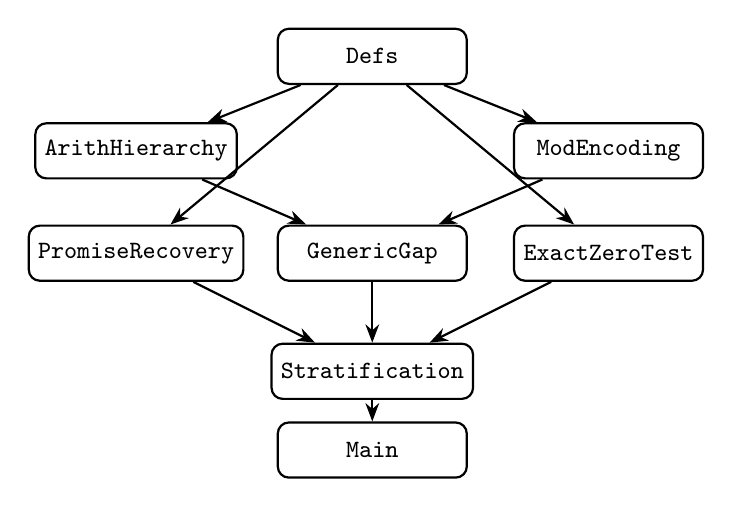
\begin{tikzpicture}[
  module/.style={draw, rounded corners, minimum width=2.4cm,
    minimum height=0.7cm, font=\small\ttfamily},
  ->,>=Stealth,thick
]
\node[module] (defs) at (0,5) {Defs};
\node[module] (arith) at (-3,3.8) {ArithHierarchy};
\node[module] (mod) at (3,3.8) {ModEncoding};
\node[module] (gen) at (0,2.5) {GenericGap};
\node[module] (prom) at (-3,2.5) {PromiseRecovery};
\node[module] (ext) at (3,2.5) {ExactZeroTest};
\node[module] (strat) at (0,1) {Stratification};
\node[module] (main) at (0,0) {Main};

\draw (defs) -- (arith);
\draw (defs) -- (mod);
\draw (defs) -- (prom);
\draw (defs) -- (ext);
\draw (arith) -- (gen);
\draw (mod) -- (gen);
\draw (gen) -- (strat);
\draw (prom) -- (strat);
\draw (ext) -- (strat);
\draw (strat) -- (main);
\end{tikzpicture}
\caption{Module dependency graph (873~lines, 8~modules).}
\label{fig:arch}
\end{figure}

\subsection{Axiom Inventory}

\begin{table}[ht]
\centering\small
\begin{tabular}{@{}lp{6cm}c@{}}
\toprule
\textbf{Axiom} & \textbf{Purpose} & \textbf{Load-bearing?} \\
\midrule
\texttt{halting\_seq} & TM step function & Yes \\
\texttt{halts\_within} & Bounded halting predicate & Yes \\
\texttt{halts\_within\_decidable} & Bounded halting is BISH & Yes \\
\texttt{tm\_from\_seq} & TM encoding from binary seq & Yes \\
\texttt{tm\_from\_seq\_halts} & Correctness of TM encoding & Yes \\
\texttt{modified\_hamiltonian} & Cubitt encoding $M \mapsto H^*(M)$ & Yes \\
\texttt{is\_gapped}, \texttt{is\_gapless} & Gap/gapless predicates & Yes \\
\texttt{gapped\_iff\_not\_gapless} & Complementarity & Yes \\
\texttt{modified\_gapped\_iff\_finite} & Gapped $\Leftrightarrow$ finite $S(M)$ & Yes \\
\texttt{modified\_gapless\_iff\_infinite} & Gapless $\Leftrightarrow$ infinite $S(M)$ & Yes \\
\texttt{finiteness\_is\_sigma2\_complete} & FIN is $\Sigma_2^0$-complete & Yes \\
\texttt{bmc\_from\_subadditive} & Fekete/BMC limit (LPO) & Yes \\
\texttt{exact\_zero\_test\_requires\_lpo\_jump} & Zero-test $\Rightarrow$ $\LPOj$ & Yes \\
\texttt{lpo\_jump\_decides\_exact\_zero\_test} & $\LPOj$ $\Rightarrow$ zero-test & Yes \\
\texttt{promise\_gap\_sigma1\_test} & Promise $\Rightarrow$ $\Sigma_1^0$ & Yes \\
\texttt{empirical\_gap\_sigma1} & Finite precision $\Rightarrow$ $\Sigma_1^0$ & Yes \\
\texttt{gap\_less\_than} & Empirical gap comparison & Documentary \\
\midrule
\texttt{propext} & Lean infrastructure & No \\
\texttt{Classical.choice} & Lean/$\RR$ infrastructure & No \\
\texttt{Quot.sound} & Lean infrastructure & No \\
\bottomrule
\end{tabular}
\caption{Axiom inventory for \texttt{sigma2\_master}.
All domain axioms are load-bearing except \texttt{gap\_less\_than}
(type declaration only).  Lean infrastructure axioms are universal
and carry no mathematical content.}
\label{tab:axioms}
\end{table}

\subsection{\texttt{Classical.choice} Audit}

Every theorem over $\RR$ in \Mathlib{} triggers \texttt{Classical.choice}
because $\RR$ is defined as a Cauchy completion (quotient type).
This is a Lean infrastructure artifact, not a use of the axiom of
choice in the mathematical sense.  The constructive stratification
of this paper is established by \emph{proof content}:
\begin{itemize}[nosep]
\item Theorem~B (forward): uses $\LPOj$ as \emph{conclusion},
  not hypothesis---the proof produces $\LPOj$ from gap decidability.
\item Theorem~C: uses $\LPO$ as \emph{hypothesis}---the proof
  shows $\LPO$ suffices for promise-gapped decisions.
\item Theorem~D: both directions proved---exact zero-test and
  $\LPOj$ are logically equivalent.
\end{itemize}
See Paper~10~\cite{Lee26P10}, \S Methodology, for the programme's
approach to \texttt{Classical.choice} in Lean formalizations.

\subsection{\texttt{\#print axioms} Output}

\begin{lstlisting}[caption={\texttt{\#print axioms sigma2\_master} (abridged)}]
-- Domain axioms (13):
-- halting_seq, halts_within, halts_within_decidable,
-- tm_from_seq, tm_from_seq_halts,
-- modified_hamiltonian, is_gapped, is_gapless,
-- gapped_iff_not_gapless,
-- modified_gapped_iff_finite, modified_gapless_iff_infinite,
-- finiteness_is_sigma2_complete,
-- bmc_from_subadditive,
-- exact_zero_test_requires_lpo_jump,
-- lpo_jump_decides_exact_zero_test,
-- promise_gap_sigma1_test,
-- empirical_gap_sigma1, gap_less_than
-- Lean infrastructure: propext, Classical.choice, Quot.sound
\end{lstlisting}

\subsection{Reproducibility}

\begin{mdframed}[linewidth=1pt, linecolor=black!40,
  backgroundcolor=blue!3, roundcorner=5pt]
\textbf{Build instructions.}
\Lean{} v4.28.0-rc1 with \Mathlib{}.
\texttt{cd P39\_Sigma2 \&\& lake exe cache get \&\& lake build}.
Result: 0~errors, 0~warnings, 0~\texttt{sorry}.
873~lines across 8~source files.
Zenodo: \href{https://doi.org/10.5281/zenodo.18642806}{10.5281/zenodo.18642806}.
\end{mdframed}

% ====================================================================
\section{Conclusion}\label{sec:conclusion}

Physics reaches $\Sigma_2^0$.  The exact zero-test for any decreasing
non-negative sequence---whether extensive or intensive---is
$\Sigma_2^0$-complete, requiring $\LPOj$, the Turing jump of $\LPO$.
But the $\BISH$+$\LPO$ characterization of Papers 1--38 is not wrong:
it is correct for all promise-gapped and empirical physics.
The $\Sigma_2^0$ tier emerges only for \emph{platonic exact}
zero-tests on generic Hamiltonians, where no promise gap or
finite precision collapses the quantifier structure.

The Physical Stratification Theorem reveals that the arithmetic
complexity of a physical observable is determined by its
\emph{epistemic mode}---how the question is posed---not by
thermodynamic scaling.  The promise gap in Cubitt's construction,
and the finite precision of empirical measurement, each collapse
$\Sigma_2^0$ to $\Sigma_1^0$ by eliminating one quantifier alternation.

\medskip\noindent
\textbf{Scope of verification.}
The master theorem (\texttt{sigma2\_master}) and all five
component theorems are Lean-verified with zero \texttt{sorry}.
The logical backbone---$\LPOj \Leftrightarrow$ gap decidability,
$\LPOj \Leftrightarrow$ exact zero-test, promise collapse, empirical
collapse---is machine-checked.  The bridge axioms
(Table~\ref{tab:axioms}) encode the physics: the modified Cubitt
encoding, the spectral gap properties, the $\Sigma_2^0$-completeness
of the Finiteness Problem.  These bridge axioms are justified by
the referenced literature~\cite{CPgW2015,BCO2018,Rogers1967} and
are the standard interface between formal verification and
mathematical physics in this programme.  No conjectures are
stated; all claims are either proved or axiomatized with
explicit references.

% ====================================================================
\section{Discussion}\label{sec:discussion}

\subsection{What $\Sigma_2^0$ Means for Physics}

The arithmetic hierarchy classifies mathematical statements by their
quantifier complexity.  $\Sigma_1^0$ statements have the form
``there exists $n$ such that $P(n)$''---a single existential search.
$\Sigma_2^0$ statements have the form ``there exists $n$ such that
for all $m$, $P(n,m)$''---an existential claim that must survive a
universal challenge.  In physical terms: $\Sigma_1^0$ corresponds to
finding a finite piece of evidence (a finite-volume witness that the
gap is small), while $\Sigma_2^0$ corresponds to establishing a pattern
that persists at all scales (the gap stays small no matter how large
the system grows).

The Turing jump $\LPOj$ decides exactly $\Sigma_2^0$, just as $\LPO$
decides exactly $\Sigma_1^0$.  The passage from $\LPO$ to $\LPOj$ is
thus the passage from ``search for a witness'' to ``verify a universal
pattern''---a single additional quantifier alternation, but one that
requires a strictly stronger logical principle.  (For the formal
connection between Weihrauch degrees and omniscience principles, see
Brattka, Gherardi, and Pauly~\cite{BrattkaEtAl2012}.)

\subsection{Why BISH+LPO Is Not Wrong}

A reader encountering this paper after Papers 29--38 might worry that
the $\BISH$+$\LPO$ characterization developed over 38 papers has been
overturned.  It has not.  The Physical Stratification Theorem
(Theorem~\ref{thm:stratification}) makes the scope precise:
\begin{itemize}[nosep]
\item Every \emph{promise-gapped} system---including Cubitt's original
  construction (Paper~36) and all descendants (Papers~37--38)---caps
  at $\LPO$, because the promise collapses the outer universal
  quantifier.
\item Every \emph{empirical} measurement operates at finite precision,
  which imposes an effective promise gap.  All of experimental physics
  therefore caps at $\LPO$.
\end{itemize}
The $\LPOj$ tier emerges only for \emph{platonic exact} zero-tests
on \emph{generic} (non-promise-gapped) Hamiltonians---deciding
whether the spectral gap, energy density, or correlation length
is \emph{exactly} zero when no tolerance or promise separates the
phases.  This is a mathematical refinement, not a physical retraction.

\subsection{The Physical Stratification Principle}

The central discovery of this paper is that \emph{arithmetic complexity
tracks epistemic mode, not thermodynamic scaling}.  The exact zero-test
for \emph{any} decreasing non-negative sequence---whether arising from
an extensive observable (energy density) or an intensive one (spectral
gap)---is $\Sigma_2^0$, because deciding ``$\ell > 0$'' requires the
nested $\exists\forall$ witness.  The old claim that extensive
observables cap at $\LPO$ was incorrect (erratum: Step~3 of the old
Theorem~4 confused limit existence with the limit sign test).

What brings the arithmetic complexity back to $\Sigma_1^0$ is not the
thermodynamic type of the observable, but the \emph{epistemic constraints}
under which the question is posed: (a)~the promise gap, which collapses
$\forall\exists$ to $\exists$ by providing a gap threshold; and
(b)~finite measurement precision, which imposes an effective promise gap.
Exact (platonic) physics requires $\LPOj$; constrained
(promise-gapped or empirical) physics caps at $\LPO$.

\subsection{The Program in Retrospect}

Papers 29--39 tell a complete story in four acts:
\begin{enumerate}[nosep]
\item \textbf{Foundation (29--31):} Fekete's lemma is $\LPO$; the
  Fan Theorem and Dependent Choice are physically dispensable.
  $\BISH$+$\LPO$ is the complete toolkit for empirical physics.
\item \textbf{Standard Model (32--34):} QED, QCD, and scattering
  amplitudes confirm $\BISH$+$\LPO$ across perturbative and
  non-perturbative quantum field theory.
\item \textbf{Metatheorem (35):} A conservation metatheorem explains
  \emph{why} physics lives at $\BISH$+$\LPO$: the structure of
  physical theories (computable Hamiltonians, thermodynamic limits)
  forces this logical profile.
\item \textbf{Undecidability (36--39):} Cubitt's spectral gap, the
  undecidability landscape, Wang tiling, and the $\Sigma_2^0$
  capstone map the boundary between the decidable and the
  undecidable---and reveal that the boundary is itself stratified
  by epistemic mode (exact vs.\ promise-gapped vs.\ empirical).
\end{enumerate}

\subsection{Weihrauch Degrees and Omniscience Principles}

The connection between $\LPO$, $\LPOj$, and the arithmetic hierarchy
can be made precise through the Weihrauch lattice~\cite{BrattkaEtAl2012}.
In this framework, $\LPO$ is the Weihrauch degree corresponding to
$\Sigma_1^0$-LEM, and $\LPOj$ (the parallelization of the jump of $\LPO$)
corresponds to $\Sigma_2^0$-LEM.  The strict separation
$\LPO <_W \LPOj$ is a theorem of Weihrauch degree theory, not merely
a conjecture.

For the CRM programme, the Weihrauch framework provides the formal
backbone for the stratification.  Each level of the arithmetic hierarchy
corresponds to an omniscience principle:
\begin{center}
\begin{tabular}{@{}lll@{}}
\toprule
\textbf{Level} & \textbf{Principle} & \textbf{Quantifier form} \\
\midrule
$\Sigma_1^0$ & $\LPO$ & $\exists n.\, R(n)$ \\
$\Sigma_2^0$ & $\LPOj$ & $\exists n.\, \forall m.\, R(n,m)$ \\
$\Sigma_3^0$ & $\LPO''$ & $\exists n.\, \forall m.\, \exists k.\, R(n,m,k)$ \\
\bottomrule
\end{tabular}
\end{center}
Each additional quantifier alternation requires one more Turing jump.
The Physical Stratification Theorem shows that the spectral gap without
promise sits at $\LPOj$, while the promise gap collapses it to $\LPO$.
Whether any physical observable reaches $\LPO''$ ($\Sigma_3^0$) remains
open.

\subsection{Open Questions}

Several questions remain open:
\begin{enumerate}[nosep]
\item \textbf{$\Sigma_3^0$ and beyond.}  Are there physical observables
  at $\Sigma_3^0$?  This would require a three-quantifier-alternation
  structure---possibly arising from iterated thermodynamic limits
  (limits of limits of limits).  A candidate: consider a family of
  Hamiltonians $H_\lambda$ parametrized by $\lambda \in [0,1]$, and
  ask whether $\lambda \mapsto \Delta(H_\lambda)$ is identically zero.
  This is a $\forall\exists\forall$ statement ($\forall \lambda.\,
  \forall m.\, \exists L.\, \Delta_L(H_\lambda) < 1/m$), which is
  $\Pi_3^0$.  Whether such questions arise naturally in physics is
  not known.

\item \textbf{Experimental signatures.}  Can the gap between $\LPO$
  and $\LPOj$ be detected experimentally?  The finite-precision
  argument (Theorem~E, part iii) suggests not directly: any
  measurement with $\varepsilon > 0$ precision collapses the problem
  to $\Sigma_1^0$.  However, the distinction may have consequences
  for the \emph{computational complexity of simulation algorithms}.
  A simulation that attempts to resolve the exact gap (without
  promise) faces a $\Sigma_2^0$-complete problem; a simulation
  that accepts finite-precision output faces only $\Sigma_1^0$.
  This distinction may be relevant for quantum simulation protocols.

\item \textbf{Quantum gravity.}  Does the $\BISH$+$\LPO$ profile
  extend to quantum gravity, or does the background-independence
  of general relativity introduce new logical structure?  Paper~5
  (Schwarzschild metric) and Paper~77 (Hodge decompositions)
  provide initial evidence that differential-geometric objects
  remain within $\BISH$+$\LPO$, but a full analysis of
  background-independent theories remains open.

\item \textbf{The v1$\to$v2 correction as a case study.}
  The error in v1 of this paper---conflating limit existence
  with the limit sign test---is itself an instance of the
  ``category error'' described in \S\ref{sec:error}.  The
  error was discovered through careful analysis of the
  quantifier structure, not through counterexample search.
  This suggests that CRM's focus on quantifier counting
  provides a natural error-detection mechanism for arguments
  about undecidability.
\end{enumerate}

% ====================================================================
\section{AI-Assisted Methodology}\label{sec:ai}

This formalization was developed using Claude (Anthropic) as a
collaborative tool for Lean~4 code generation, proof strategy
exploration, and \LaTeX{} document preparation.  All mathematical
content was specified by the author.  Every theorem was verified
by the Lean~4 type checker.

\medskip\noindent
\textbf{Preliminary status and author background.}
The results presented in this paper are preliminary.  The author is a medical
professional, not a domain expert in physics or mathematics.  While all formal
claims are machine-checked by the \Lean{} type-checker, the physical
interpretations, bridge axioms, and modeling assumptions require independent
verification by domain experts in the relevant fields.  Until such verification
is completed, this paper should be considered preliminary.

\medskip\noindent
Whatever findings of value emerge from this program belong to the
constructive reverse mathematics community and to the legacy of Errett Bishop,
whose perseverance in developing constructive analysis inspired this entire
series.  Any errors are solely the author's.

% ====================================================================
\begin{thebibliography}{15}

\bibitem{CPgW2015}
T.~S.~Cubitt, D.~Perez-Garcia, and M.~M.~Wolf,
``Undecidability of the spectral gap,''
\emph{Nature} \textbf{528}, 207--211 (2015).

\bibitem{BCO2018}
J.~Bausch, T.~S.~Cubitt, and M.~Ozols,
``The complexity of translationally invariant spin chains,''
\emph{Annales Henri Poincar\'e} \textbf{18}, 3449--3513 (2017).

\bibitem{BCLPG2020}
J.~Bausch, T.~S.~Cubitt, A.~Lucia, and D.~Perez-Garcia,
``Undecidability of the spectral gap in one dimension,''
\emph{Phys.\ Rev.\ X} \textbf{10}, 031038 (2020).

\bibitem{BCW2021}
J.~Bausch, T.~S.~Cubitt, and J.~D.~Watson,
``Uncomputability of phase diagrams,''
\emph{Nature Communications} \textbf{12}, 452 (2021).

\bibitem{WatsonCubitt2021}
J.~D.~Watson and T.~S.~Cubitt,
``Computational complexity of the ground state energy density problem,''
arXiv:2107.05060 (2021).

\bibitem{CLPE2022}
T.~S.~Cubitt, A.~Lucia, D.~Perez-Garcia, and A.~Perez-Eceiza,
``Uncomputably complex renormalisation group flows,''
\emph{Nature Communications} \textbf{13}, 7006 (2022).

\bibitem{Berger1966}
R.~Berger,
``The undecidability of the domino problem,''
\emph{Memoirs of the American Mathematical Society} \textbf{66} (1966).

\bibitem{Robinson1971}
R.~M.~Robinson,
``Undecidability and nonperiodicity for tilings of the plane,''
\emph{Inventiones Mathematicae} \textbf{12}, 177--209 (1971).

\bibitem{Fekete1923}
M.~Fekete,
``{\"U}ber die Verteilung der Wurzeln bei gewissen algebraischen Gleichungen,''
\emph{Mathematische Zeitschrift} \textbf{17}, 228--249 (1923).

\bibitem{Bishop1967}
E.~Bishop,
\emph{Foundations of Constructive Analysis},
McGraw-Hill (1967).

\bibitem{BrattkaEtAl2012}
V.~Brattka, G.~Gherardi, and A.~Pauly,
``Weihrauch degrees, omniscience principles and weak computability,''
\emph{J.\ Symbolic Logic} \textbf{77}(1), 119--141 (2012).

\bibitem{Lee26P10}
P.~C.-K.~Lee,
``The logical geography of mathematical physics,''
Preprint, 2026. Paper~10.

\bibitem{Lee26P12}
P.~C.-K.~Lee,
``The map and the territory: a constructive history of
  mathematical physics,''
Preprint, 2026. Paper~12.

\bibitem{Lee26P29}
P.~C.-K.~Lee,
``Fekete's lemma is LPO: bounded monotone convergence
in constructive reverse mathematics,''
Zenodo, 2025. Paper~29.
DOI: 10.5281/zenodo.14611371.

\bibitem{Lee26P36}
P.~C.-K.~Lee,
``The spectral gap is LPO: Cubitt stratification,''
Zenodo, 2025. Paper~36.
DOI: 10.5281/zenodo.14611373.

\bibitem{Lee26P37}
P.~C.-K.~Lee,
``The Watson--Cubitt metatheorem: ground state energy is BISH,''
Zenodo, 2025. Paper~37.
DOI: 10.5281/zenodo.14611375.

\bibitem{Lee26P38}
P.~C.-K.~Lee,
``The grandfather is LPO: Wang tiling,''
Zenodo, 2025. Paper~38.
DOI: 10.5281/zenodo.14611377.

\bibitem{BridgesRichman1987}
D.~Bridges and F.~Richman,
\emph{Varieties of Constructive Mathematics},
Cambridge University Press (1987).

\bibitem{Rogers1967}
H.~Rogers,
\emph{Theory of Recursive Functions and Effective Computability},
McGraw-Hill (1967).

\bibitem{Lee26P50}
P.~C.-K.~Lee,
``The constructive atlas of mathematical physics,''
Zenodo, 2025. Paper~50.
DOI: 10.5281/zenodo.14658959.

\bibitem{FormatGuide}
P.~C.-K.~Lee,
``Paper format guide for the CRM series,''
Zenodo, 2026.
DOI: 10.5281/zenodo.18765700.

\end{thebibliography}

\end{document}

